\section{Защита данных в распределенных системах}
\subsection{Распределенные вычислительные среды}
Распределённая обработка данных - методика выполнения прикладных программ группой систем.
При этом пользователь получает возможность работать с сетевыми службами и прикладными процессами,
расположенными в нескольких взаимосвязанных абонентских системах. \autocite{Sergeeva}

\paragraph{
    Распределенная обработка информации в среде клиент-сервер.
    Концепция распределенной вычислительной среды Distributed Computing Environment (DCE).
    Распределенные базы данных в сетях ЭВМ
} ~\\

Компьютер (или программу), управляющий ресурсом, называют сервером этого ресурса (файлсервер, сервер базы данных,
вычислительный сервер...). Клиент и сервер какого-либо ресурса могут находиться как в рамках одной вычислительной системы,
так и на различных компьютерах, связанных сетью. Основной принцип технологии "клиент-сервер" заключается в разделении
функций приложения на три группы:
\begin{itemize}
    \item ввод и отображение данных (взаимодействие с пользователем);
    \item прикладные функции, характерные для данной предметной области;
    \item функции управления ресурсами (файловой системой, базой данных и т.д.)
\end{itemize}

Поэтому, в любом приложении можно выделить следующие компоненты:
\begin{itemize}
    \item компонент представления данных
    \item прикладной компонент
    \item компонент управления ресурсом
\end{itemize}

Связь между компонентами осуществляется по определенным правилам, которые называют "протокол взаимодействия".
Каждый из компонентов приложения при этом может работать на выделенном сервере (узле) или разделять ресурсы сервера
с другими компонентами приложения. В связи с этим можно выделить следующие модели приложений:
\begin{itemize}
    \item двухзвенная модель (модель «клиент-сервер»)
    \item трехзвенная модель (модель сервера приложений)
    \item многозвенная модель
\end{itemize}

\textbf{Двухзвенная модель} позволяет распределить различным образом три компонента приложения между двумя узлами.
\textbf{Трехзвенная модель} предполагает выделение для каждого из трех компонентов приложения свой сервер.
\textbf{Многозвенная модель} позволяет отдельным компонентам использовать ресурсы нескольких серверов, например,
распределенные базы данных. Компанией Gartner Group, специализирующейся в области исследования информационных технологий,
предложена следующая классификация двухзвенных моделей взаимодействия клиент-сервер \autocite{dce}
\begin{figure}[h!]
    \centering
    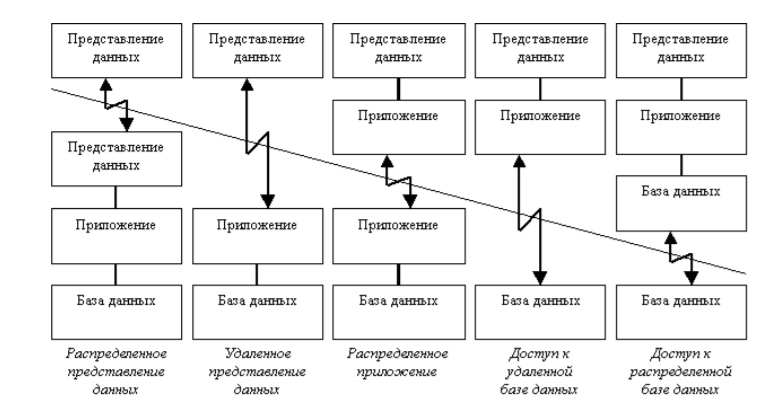
\includegraphics[width=0.8\textwidth]{assets/dce.jpg}
    \caption{Классификация двухзвенных моделей}
\end{figure}
\\

\subsection{Угрозы безопасности распределенных СУБД}
\paragraph{Угрозы доступности, целостности и конфиденциальности данных. Механизмы противодействия} ~\\

В данном материале \autocite{infosec} предпринята попытка изложить комплексный подход к обеспечению безопасности
распределенных информационных систем (ИС).
Однако в рамках одной статьи не представляется возможным подробно описать все аспекты информационной безопасности,
поэтому поднятые вопросы рассмотрены очень кратко. Однако были приложены все усилия к тому,
чтобы не упустить ни одну из проблем так или иначе влияющую на безопасность ИС.

При рассмотрении информационной безопасности распределенных ИС выбран клиент/серверный подход, ввиду того,
что он позволяет провести декомпозицию ИС на отдельные компоненты, обеспечивающие определенные сервисы,
а также потому, что ряд услуг по безопасности может быть реализован в виде отдельных серверов.

Кроме этого необходимо отметить, что обеспечение абсолютной защищенности информации
в распределенных ИС - задача, практически, не достижимая, что обусловлено не только техническими вопросами,
но и человеческим фактором. Поэтому вопрос может стоять только об определенном уровне защищенности.

\bigbreak
\textbf{Современный подход к информационной безопасности}

Под информационной безопасностью понимается защита информации и поддерживающей ее инфраструктуры с помощью
совокупности программных, аппаратно-программных средств и методов, а также организационных мер, с целью недопущения
причинения вреда владельцам этой информации или поддерживающей ее инфраструктуре.

При построении системы защиты должен учитываться комплексный подход в обеспечении безопасности информации.
Он подразумевает использование защитных механизмов на всех этапах жизненного цикла системы, от ее проектирования
и до вывода из эксплуатации, и совместное решение целого спектра вопросов, начиная от физической защиты объектов ИС,
с применением интеллектуальной системы контроля доступа, и заканчивая вопросами поддержки нормального функционирования
ИС в критических ситуациях.

Проектирование системы безопасности информации (СБИ) осуществляется совместно с проектированием самой информационной системы.
При внесении любых изменений в структуру ИС, это должно найти адекватное отражение и в системе защиты.

При разработке систем информационной безопасности необходимо учитывать передовые тенденции развития информационных
технологий, к каким в настоящее момент относятся интрасети (Интранет - Intranet).
Характерными чертами данных сетей является то, что они основываются на технологии клиент/сервер, имеют в своем составе
разнородные корпоративные информационные системы и пользуются внешними сервисами, базовым для которых является
протокол TCP/IP, а также предоставляет аналогичные сервисы вовне. Центральным элементом интрасетей является
WEB-сервис, поэтому чрезвычайно важным является вопрос обеспечения защищенности этого сервиса.

\bigbreak
\textbf{Разработка политики безопасности}

Первым шагом на пути построения СБИ является разработка политики безопасности ИС.
Под политикой безопасности следует понимать утвержденный высшим должностным лицом организации, в
интересах которой разрабатывается ИС и система защиты, документ, с указанием организационных и технических мероприятий,
направленных на защиту информации, и поддерживающей ее инфраструктуры.

В данном документе должны найти обязательное отражение основные принципы безопасности информации,
такие как многоуровневая защита и разнообразие средств и методов защиты, минимизация привилегий, разделение полномочий,
невозможность обхода средств защиты и т.п.

\bigbreak
\textbf{Построение модели нарушителя}

После разработки политики безопасности производится анализ угроз ИС, возможных каналов утечки информации и
построение на этой основе модели потенциального нарушителя.

Согласно предлагаемой модели, в качестве нарушителя может выступать как отдельное физическое лицо,
так и специальные программы, содержащие в себе некие деструктивные элементы - разрушающие программные компоненты (РПК).

Под объектом защиты в данной модели понимается материальный носитель защищаемой информации, а также сама информация,
доступ к которым определен режимом разграничения доступа, реализуемым системой защиты, а также поддерживающая инфраструктура.

Предполагается, что по отношению к ИС нарушитель может быть двух типов: внутренним или внешним.
При этом внутренний нарушитель выступает в качестве законного пользователя системы или лица из числа
обслуживающего персонала или администрации ИС, а внешний является лицом, не подпадающим ни под
одну из указанных категорий. РПК, в свою очередь, может быть отнесено к категории внутреннего нарушителя.

Возможные угрозы нарушителя напрямую зависят от его типа. Возможности внутреннего нарушителя ограничены
установленными правилами разграничения доступа, внутриобъектовым режимом и его функциональными обязанностями.
Возможности РПК в ИС намного шире и определяются работоспособностью ПО, в котором они заложены,
а также наличием в системе средств активного аудита и мониторинга.

\bigbreak
\textbf{Проектирование СБИ}

Следующим шагом после разработки модели нарушителя является проектирование СБИ.
Согласно принципу многоуровневой защиты и разнообразия средств и методов защиты, можно выделить следующие
самостоятельные системы в составе СБИ (при этом необходимо учитывать, что все они интегрированы
и находятся в тесной взаимосвязи):
\begin{itemize}
    \item Система контроля доступа на объекты и в помещения ИС
    \item Система защиты информации в ИС от НСД
    \item Средства защиты от РПК
    \item Средства поддержания доступности информации в ИС
\end{itemize}

\bigbreak
\textbf{Система контроля доступа}

Система контроля доступа на объекты и в помещения, в которых функционирует ИС, должна состоять из трех подсистем:
пропускная подсистемы (ПП), подсистемы охранной сигнализации (ПОС) и подсистемы телевизионного наблюдения (ПТН).

Простейшим вариантом пропускной подсистемы являются одиночные кодовые замки, устанавливаемые в защищаемых помещениях,
либо электронные замки с карточками доступа - ЭЗКД. Учитывая, что в ЭЗКД предусмотрен режим постановки
на охрану, то ПП может быть интегрирована с ПОС.

Что касается ПОС и ПТН, то они не отделимы одна от другой и функционируют под управлением единого вычислительного комплекса.

\bigbreak
\textbf{Система защиты информации в ИС от НСД}

Данная система может быть реализована как встроенными средствами защиты сетевых операционных
систем и систем управления базами данных (СУБД), так и дополнительными средствами. Стоит лишь отметить,
что при построении системы защиты от НСД необходимо, по возможности, избегать дублирования многих функций,
с тем, чтобы СБИ не страдала избыточностью, что в конечном итоге скажется как на удобстве работы
пользователей и их желании выполнять все предписания системы защиты, так и на управляемости самой СБИ.

В состав указанной системы также должны входить:
\begin{itemize}
    \item средства контроля, управления и идентификации при удаленном доступе
    \item средства управления доступом и идентификации в рамках ИС
    \item средства экранирования ИС от открытых сетей, а также разноуровневых сетей внутри данной ИС друг от друга
    \item средства управления, анализа и аудита СБИ в рамках сетевых конфигураций
\end{itemize}

\bigbreak
\textbf{Средства контроля, управления и идентификации при удаленном доступе к ИС}

Указанная категория средств предназначена для осуществления процедуры контроля подключения к ИС удаленных пользователей,
а также для управления их доступом и осуществления идентификации. Данная проблема возникает в связи со структурой
интрасетей, когда удаленные пользователи получают доступ к ресурсам корпоративной ИС по выделенным,
либо коммутируемым каналам связи. В этом случае существует реальная вероятность несанкционированного подключения
нарушителя к линии связи, с активным или пассивным прослушиванием сети и выдачей себя за
регистрированного пользователя ИС. В целях недопущения подобного целесообразно применение методов с
использованием одноразовых паролей и единого входа в сеть

Принцип систем с одноразовыми паролями основан на однократном использовании пароля для процедуры
идентификации в ИС, в результате чего перехват его нарушителем становится бессмысленным.
Идентификация и аутентификация пользователя осуществляется сервером безопасности (аутентификации), входящим в состав ИС.

Концепция единого входа в сеть предоставляет существенное удобство для пользователей, так как при
подключении к ИС им достаточно только один раз доказать свою подлинность. Кроме этого, применение
этой концепции способствует усилению информационной безопасности, ввиду того, что в сети
отсутствует открытая передача аутентификационной информации.

\bigbreak
\textbf{Средства управления доступом и идентификации в рамках ИС}

Учитывая территориальную разнесенность современных ИС и использование технологии клиент/сервер, целесообразно выделение функции проверки подлинности в виде отдельного сервера безопасности (аутентификации). Услугами данного сервера должны пользоваться все другие серверы и пользователи ИС.

Сервер безопасности может быть реализован в виде одного или нескольких серверов, функционирующих на физически защищенных компьютерах. Серверы должны содержать репозиторий субъектов ИС и их секретные ключи.

При построении сервера безопасности возможны два пути:
\begin{itemize}
    \item Сервер безопасности с центральным хранением данных репозитория
    \item Сервер безопасности с децентрализованным хранением данных репозитория
\end{itemize}

Однако централизованное хранение является нецелесообразным по следующим причинам:
\begin{itemize}
    \item сильная зависимость от готовности сервера
    \item возможность расширения или комбинирования сетей в процессе развития ИС
\end{itemize}

Дополнительной причиной децентрализации сервера безопасности является объединение сетей при развитии ИС. Возможна ситуация, когда две до того независимые сети, имеющие каждая в своем составе отдельный сервер безопасности, объединяются. В этом случае один из серверов должен быть уничтожен, а все определенные в нем данные по авторизации переданы на другой сервер. Если же связь между двумя сетями устанавливается временно, то необходимо наличие нескольких серверов безопасности. В противном случае, один сервер должен будет производить постоянные, двойные определения то для одной, то для другой сети. Для того, чтобы избежать этого, необходимо наличие нескольких серверов безопасности.

\bigbreak
\textbf{Средства экранирования ИС}

Средства экранирования используются для подключения ИС к открытым сетям или развязки разноуровневых сетей, т.е. сетей, обрабатывающих информацию с различным грифом секретности. Концепция систем типа Firewall (брандмауер, межсетевой экран) была разработана для снижения риска нелегального доступа к закрытой информации при подключении частных сетей (в том числе ЛВС) к сетям общего пользования. Межсетевой экран представляет собой программно-аппаратный комплекс, размещенный на стыке двух сетей и реализующий следующие три функции:
\begin{itemize}
    \item обеспечение обмена данными между сетями только через указанную систему
    \item фильтрация трафика обмена
    \item предотвращение возможности проникновения в сам экран
\end{itemize}

В этом случае обеспечивается эффективная блокировка внешнего трафика частной сети и жесткий контроль за ним. Кроме того экраны могут осуществлять разграничение доступа между различными сегментами одной корпоративной сети, а также контроль за информационными потоками, направленными во вне, обеспечивая тем самым необходимый режим конфиденциальности.

Применение экранов также позволяет существенно уменьшить уязвимость внутренних сервисов безопасности, так как нарушителю необходимо вначале преодолеть защитные механизмы самого экрана, где они сконфигурированы особенно тщательно.

Существующие в настоящее время экраны могут быть условно разделены на следующие четыре типа:
\begin{itemize}
    \item экраны с фильтрацией пакетов (packet-filtering firewall)
    \item шлюзы сеансового уровня (circuit-level gateway)
    \item шлюзы прикладного уровня (application-level gateway)
    \item экраны экспертного уровня (stateful inspection firewall)
\end{itemize}

Однако лишь некоторые экраны могут быть отнесены только к одной из указанный категорий. При этом необходимо отметить, что экраны экспертного уровня обеспечивают один из самых высоких на сегодняшний день уровней безопасности интрасетей.

\bigbreak
\textbf{Средства управления, анализа и аудита}

Средства аудита занимают свое особое положение в ряду средств обеспечения безопасности информации, заключающееся в том, что все действия нарушителя по преодолению средств защиты фиксируются, позволяя тем самым вовремя обнаружить попытку несанкционированного входа в ИС. Причем, учитывая принцип многоуровневой защиты, нарушителю придется преодолевать несколько защитных рубежей, что будет обязательно отмечено в регистрационном протоколе. В случае если указанная процедура выполняется в режиме реального времени, администратором безопасности могут быть своевременно предприняты соответствующие меры по предотвращению незаконного вторжения на одном из следующих уровнях защиты.

Кроме средств аудита часть программных продуктов также позволяет осуществлять оценку системы безопасности сети, имитируя все известные способы, применяемые нарушителями для проникновения в интрасети, и тем самым, обнаруживая в системе защиты слабые места. Данные программные продукты не только выявляют уязвимые места, но и определяют действия, которые необходимо предпринять для ликвидации пробелов в сетевой системе безопасности. Администратору остается лишь выбрать способы их устранения.

\bigbreak
\textbf{Средства защиты от РПК}

Учитывая, что среди отнесенных к РПК компонентов особое распространение получили компьютерные вирусы, в данном разделе описывается подход по осуществлению антивирусной защиты в ИС.

Так как сети, построенных по технологии Интранет, являются разнородными системами, важную роль приобретает использование антивирусных средств (ABC), изначально ориентированных на работу в сети и поддерживающих многоплатформность. В связи с этим особую актуальность приобретает использование ABC, предназначенных для работы в смешанных сетях NetWare и Windows NT. Наряду с этим, учитывая, что ключевым сервисом интрасетей является WEB-сервис, возникает необходимость применения антивирусного сканера, предназначенного для осуществления проверки наличия вирусов в файлах, загружаемых программами просмотра WEB-страниц (WEB-броузерами), получаемых с FTP-серверов и в почтовых сообщениях, действуя совершенно прозрачно для пользователей. Активизация ABC происходит автоматически при запуске WEB-броузера.

Особенности организации защиты информации от компьютерных вирусов

Система защиты от вирусов должна строиться исходя из обязательного выполнения следующих процедур:
\begin{itemize}
    \item входной контроль новых программных средств и входной контроль поступающей по сети информации и данных (выполняется применяемыми ABC)
    \item защиту операционной системы и системных программ от заражения (создание ABC типа ViruSaf е Multi-LAN специальной аварийной дискеты с COMMAND.COM, IPX и NETX)
    \item карантинный режим эксплуатации нового программного обеспечения
    \item резервирование главной загрузочной записи (MBR), таблицы размещения файлов (FAT) и CMOS-памяти (применение ABC ViruSafe Multi-LAN, IncoluLAN и т.п.)
\end{itemize}

\bigbreak
\textbf{Средства резервного копирования}

Резервное копирование программ и данных необходимо проводить с целью минимизации потерь в случае отказов оборудования, либо сбоев в программном обеспечении ИС. Данная задача наиболее сложна именно в интрасетях с их распределенными ресурсами и неоднородностью, в которых работают компьютеры под управлением различных операционных систем. Учитывая клиент/серверный характер интрасетей функцию резервного копирования целесообразно также выделить в виде отдельного сервера (сервера архива).

Распространение клиент/серверного подхода на процедуру резервного копирования информации и данных имеет ряд преимуществ по сравнению с традиционными методами. Они выражаются в следующем:
\begin{itemize}
    \item Администраторы рабочих групп освобождаются от необходимости согласования действий и самой процедуры создания локальных резервных копий
    \item Единообразие процедуры создания резервных копий в ИС
    \item Возможность мониторинга процесса резервирования и диагностики возникших проблем
\end{itemize}

Одним из способов обеспечения высокой доступности информации является создание резервных копий с возможностью ее хранения в двух местах: один экземпляр хранится поблизости от оригинала, а другой в удаленном безопасном месте.

\bigbreak
\textbf{Безопасность систем управления базами данных}

Составной частью информационной безопасности ИС является безопасность систем управления базами данных (СУБД). Учитывая, что СУБД является ключевым элементом современной ИС, можно отметить, что для них важны все три аспекта информационной безопасности: конфиденциальность, целостность и доступность.

В СУБД для идентификации и проверки подлинности применяются либо соответствующие механизмы операционной системы, либо специальный SQL-оператор.

\bigbreak
\textbf{Обеспечение конфиденциальности данных}

В СУБД, как правило, используется произвольное управление доступом, когда владелец объекта передает права доступа к нему (привилегии) по своему усмотрению. При этом привилегии в СУБД можно подразделить на две категории: привилегии безопасности и привилегии доступа.

Привилегии безопасности всегда выделяются конкретному пользователю и позволяют выполнять административные действия.

Привилегии доступа определяют права доступа субъектов к определенным объектам.

Специфическим механизмом управления доступом в СУБД являются представления. Они позволяют сделать видимыми для субъектов только те столбцы базовых таблиц, доступ к которым предоставлен субъектам администратором базы.

\bigbreak
\textbf{Поддержание целостности}

Целостность данных не менее важна, чем конфиденциальность, ввиду того, что для баз данных, как и для ИС в целом, главными врагами являются не внешние нарушители, а ошибки оборудования, программ, администраторов и пользователей системы.

С точки зрения пользователей СУБД, основными средствами поддержания целостности данных являются ограничения и правила.

Ограничения могут относиться как к таблицам, так и к отдельным столбцам. Они накладываются владельцами таблицы и оказывают влияние на все операции с данными.

Правила позволяют вызывать выполнение заданных действий при определенных изменениях базы данных. В отличие от ограничений, являющихся лишь средствами контроля простых условий, правила позволяют создавать сколь угодно сложные соотношения между различными элементами базы данных.

\bigbreak
\textbf{Обеспечение доступности данных}

Доступность данных подразумевает обеспечение информационной системы средствами поддержания высокой доступности. Поддержание высокой доступности позволяет свести к минимуму возможные сбои аппаратного обеспечения, в частности носителей информации, а также ошибки обслуживающего персонала и программного обеспечения. В качестве мер поддержания высокой доступности может быть названа кластеризация сервера баз данных (выделение нескольких компьютеров, выполняющих общее приложение), а также тиражирование данных (хранение базы данных в различных местах).

\bigbreak
\textbf{Угрозы СУБД}

СУБД отличаются от других компонентов ИС специфичными угрозами, и главным их источником является сама природа баз данных. Известно, что основным средство общения с СУБД выступает язык SQL, являющийся мощным инструментом манипулирования данными. С его помощью, используя механизм правил, могут быть созданы сложные, трудно поддающиеся анализу цепочки действий, позволяющие не явным образом передавать право на выполнение определенных процедур тем, кто не имеет на это полномочий.

В качестве примера можно привести несколько угроз, возникающих при использовании языка SQL: получение информации путем логических выводов, агрегирование данных, покушение на высокую доступность.

Методы борьбы против получения информации путем логических выводов состоят в тщательном проектировании модели данных, иерархии привилегий и видимых пользователям представлений.

Агрегирование данных состоит в получении новой информации путем комбинирования данных, полученным официальным путем. Причем информация, содержащаяся в скомбинированных данных, может иметь гриф более высокий, чем первичная информация.

Методом борьбы с агрегированием может быть тщательное проектирование модели данных и максимально допустимое ограничение доступа пользователей к информации.

Покушение на высокую доступность может быть реализовано, если пользователю-нарушителю доступны все возможности языка SQL. При этом он легко сможет заблокировать работу других пользователей. Поэтому, в целях борьбы с данным видом угроз, рекомендуется запрещать непосредственный SQL-доступ к базе данных, используя для этого серверы приложений.


\subsection{Распределенная обработка данных}
\paragraph{Понятие распределенной транзакции}
\paragraph{Модель обработки транзакций}
\paragraph{Мониторы обработки транзакций}
\paragraph{Корпоративная среда обработки транзакций}

\subsection{Протоколы фиксации}
\paragraph{Протоколы фиксации}
\paragraph{Защищенные протоколы фиксации}
\paragraph{Обработка распределенных транзакций в базах данных с многоуровневой секретностью (MLS)}

\subsection{Тиражирование данных}
\paragraph{Обзор средств тиражирования данных}
\paragraph{Эффективные алгоритмы тиражирования}
\paragraph{Сравнение подходов к тиражированию БД}

\subsection{Интеграция БД и Internet}
\paragraph{Современные тенденции}
\paragraph{Обзор существующих технологий}
\paragraph{Вопросы безопасности: угрозы и методы противодействия}
\paragraph{Перспективы развития}